\chapter{Phân tích thiết kế hệ thống}
\section{Tổng quan các chức năng}
\subsection{Biểu đồ use case tổng quan}
\begin{figure}[H]
    \centering
    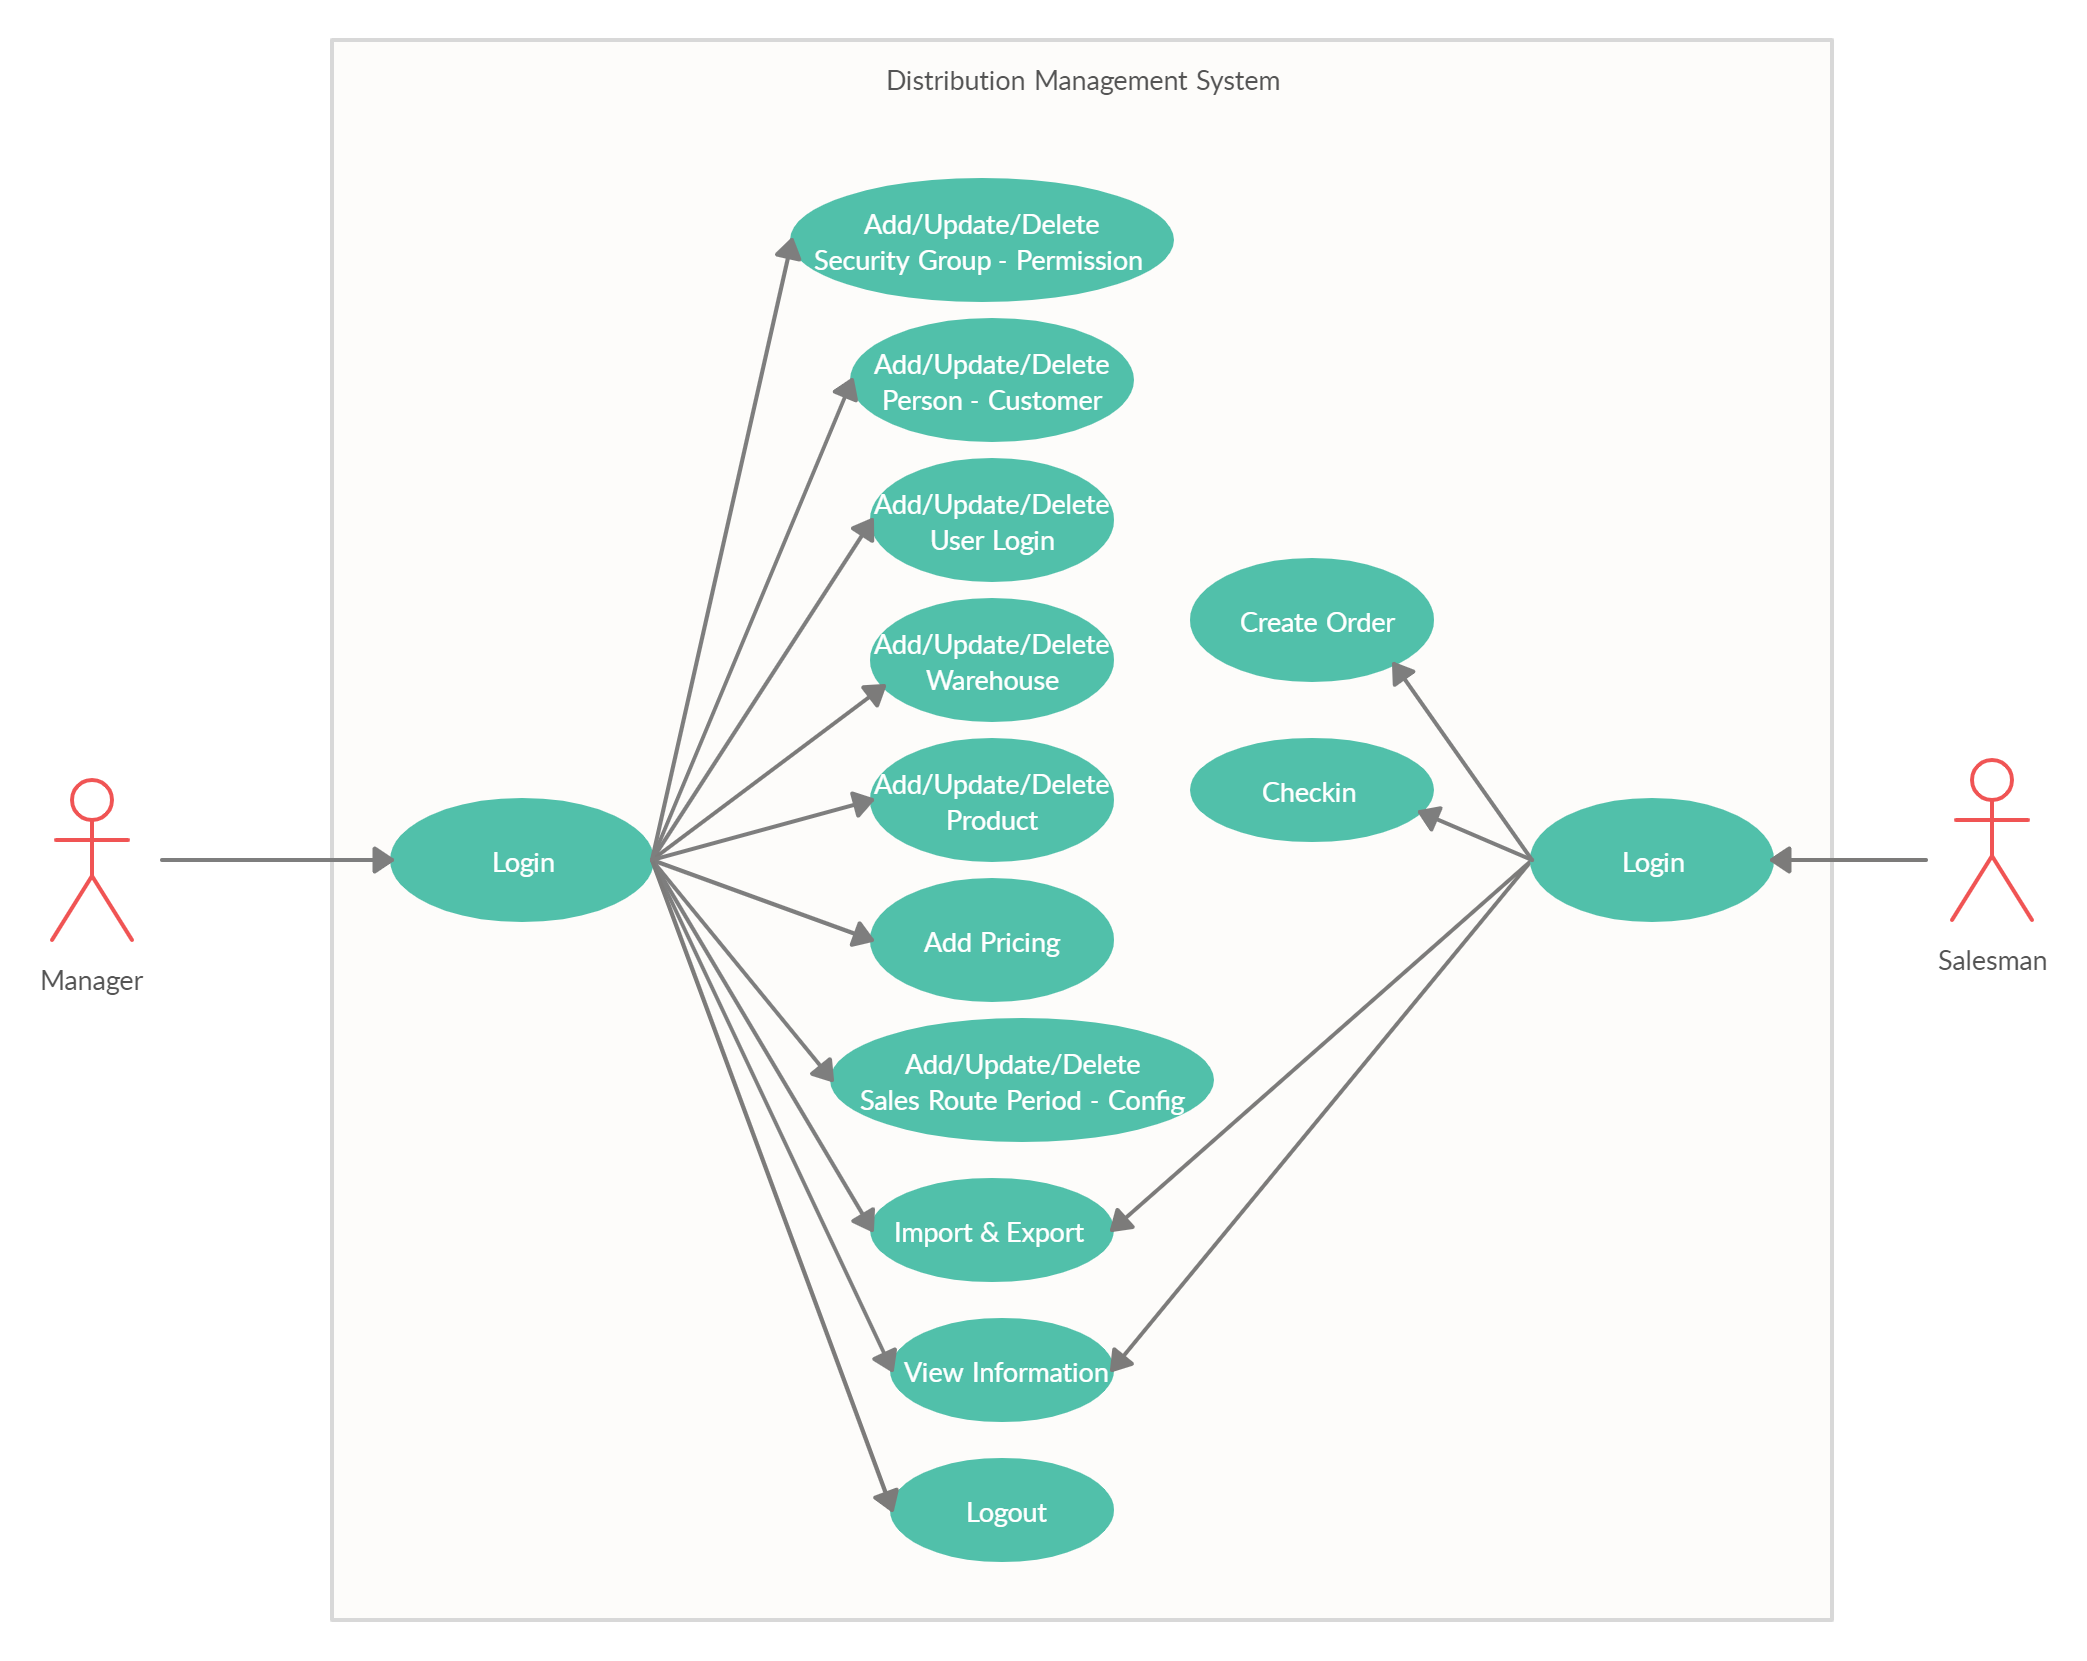
\includegraphics[width=12cm]{images/use-case/use-case-summary.jpg}
    \caption{Biểu đồ use case tổng quan}
\end{figure}

Hai tác nhân chính trong biểu đồ use case tổng quan
là người quản lý (manager) và nhân viên bán hàng (salesman).
Người quản lý ở đây là từ dùng chung, đại diện cho những người
quản lý nghiệp vụ riêng (quản lý sản phẩm, quản lý hàng tồn kho,
quản lý kho, quản lý giao dịch, quản lý tuyến bán hàng).
Người quản lý sau khi đăng nhập vào hệ thống có thể thực hiện
các nghiệp vụ quản lý như thêm / sửa / xóa sản phẩm, người dùng, …
Nhân viên bán hàng sau khi đăng nhập có thể xem được lịch
trình di chuyển của mình, lên hóa đơn mua hàng, check-in.

\subsection{Biểu đồ use case phân rã các chức năng của hệ thống}
Trong phần này, em sẽ trình bày các ca sử dụng chính trong hệ
thống, đưa ra biểu đồ use case và biểu đồ hoạt động chỉ cách
thức tương tác của người dùng với giao diện hệ thống. Do nhiều thao
tác có tính chất tương đồng nên em sẽ đưa ra các biểu
đồ hoạt động điển hình, các thao tác khác được thực hiện tương tự.

\subsubsection{Quản lý người dùng và phân quyền}
Biểu đồ use case cho ca sử dụng quản lý người dùng

\begin{figure}[H]
\centering
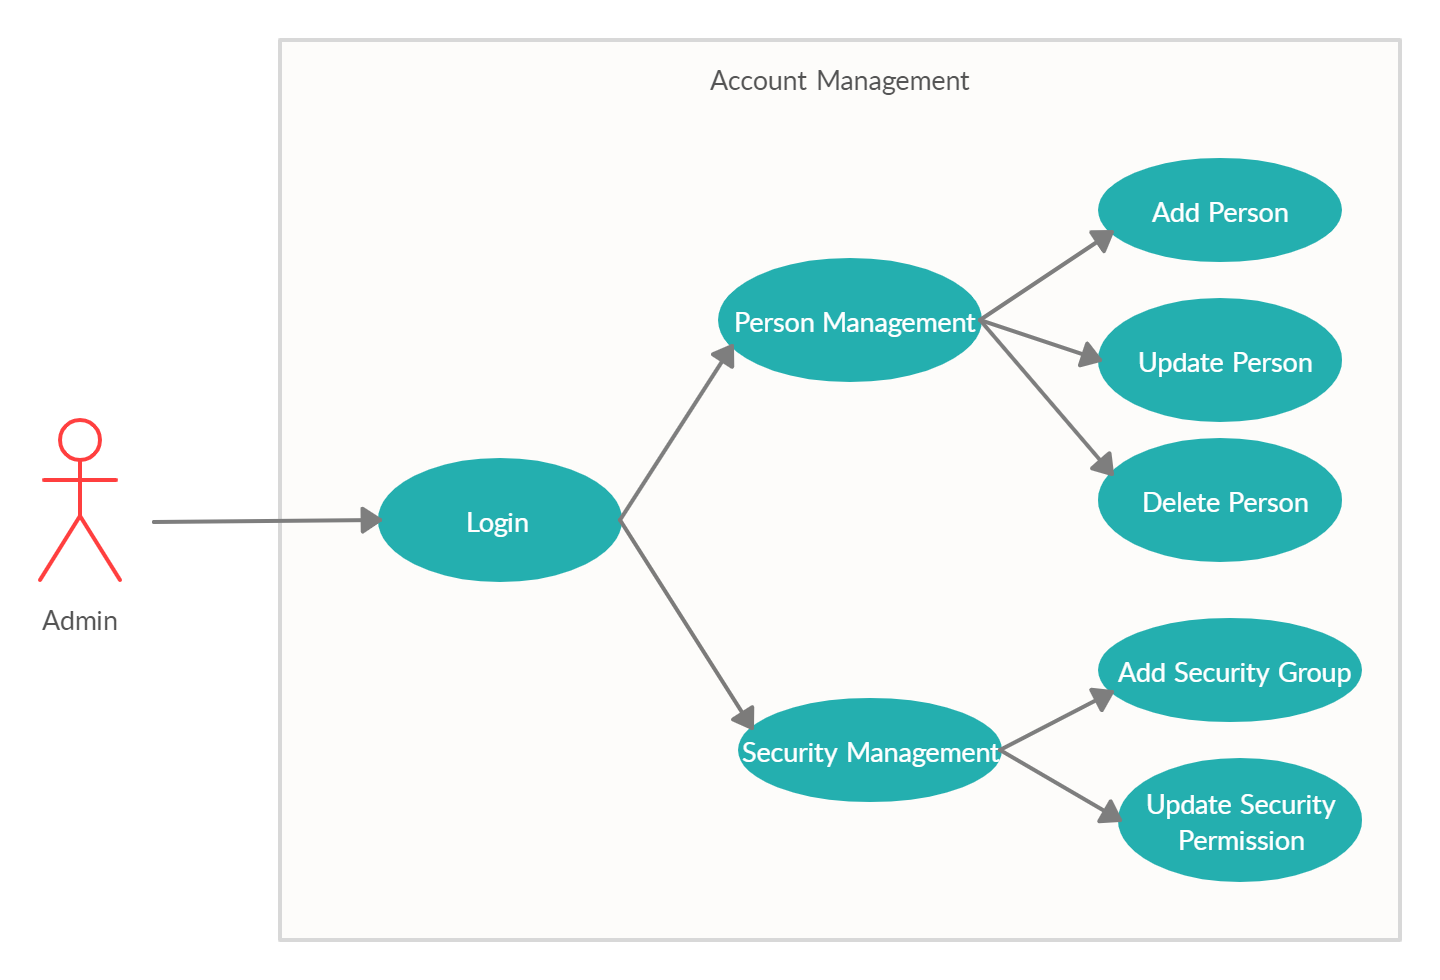
\includegraphics[width=12cm]{images/use-case/account-management.jpg}
\caption{Use-case quản lý người dùng}
\end{figure}

Người quản trị (admin) có thể quản lý các người dùng trong
hệ thống, quản lý quyền hạn của người dùng. Có thể thêm / sửa /
xóa người dùng, khách hàng, thêm / sửa quyền cho các người
quản lý cấp dưới.


Biểu đồ hoạt động cho các thao tác trong quản lý người dùng:
\begin{figure}[H]
\centering
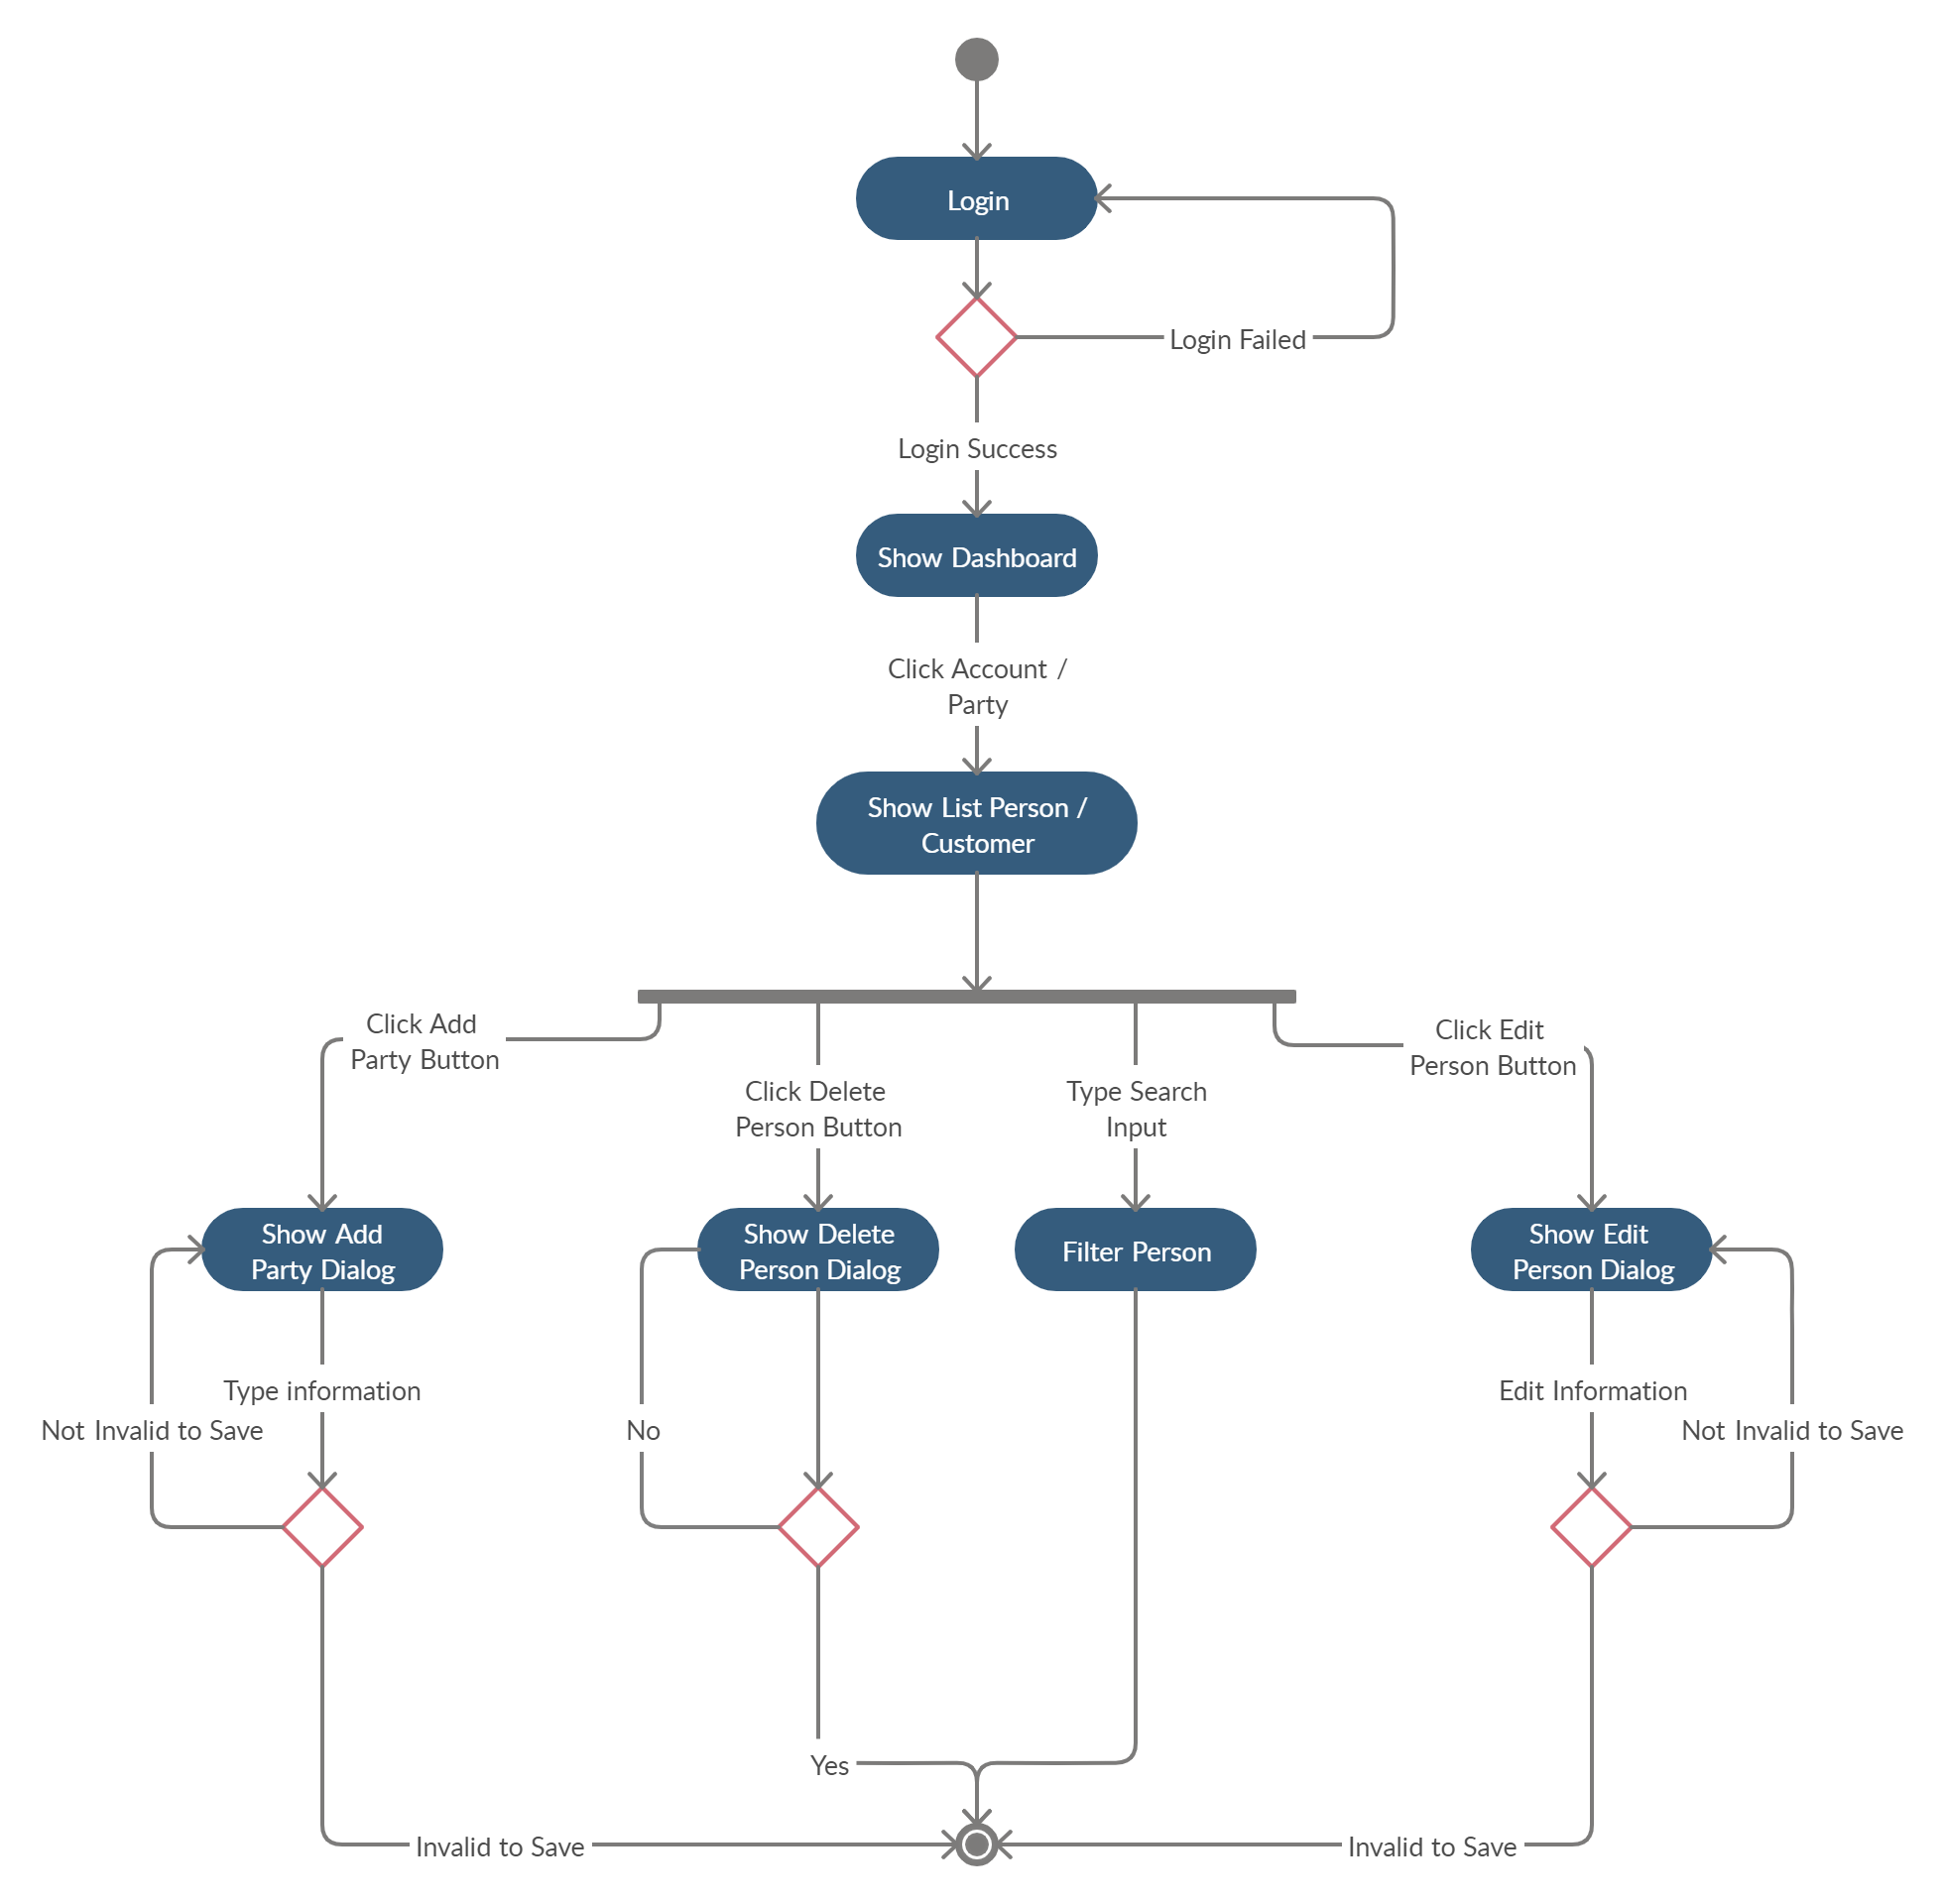
\includegraphics[width=15cm]
{images/activity-diagram/account-management.png}
\caption{Biểu đồ hoạt động ca sử dụng quản lý người dùng}
\end{figure}

Biểu đồ hoạt động cho thao tác phân quyền:
\begin{figure}[H]
\centering
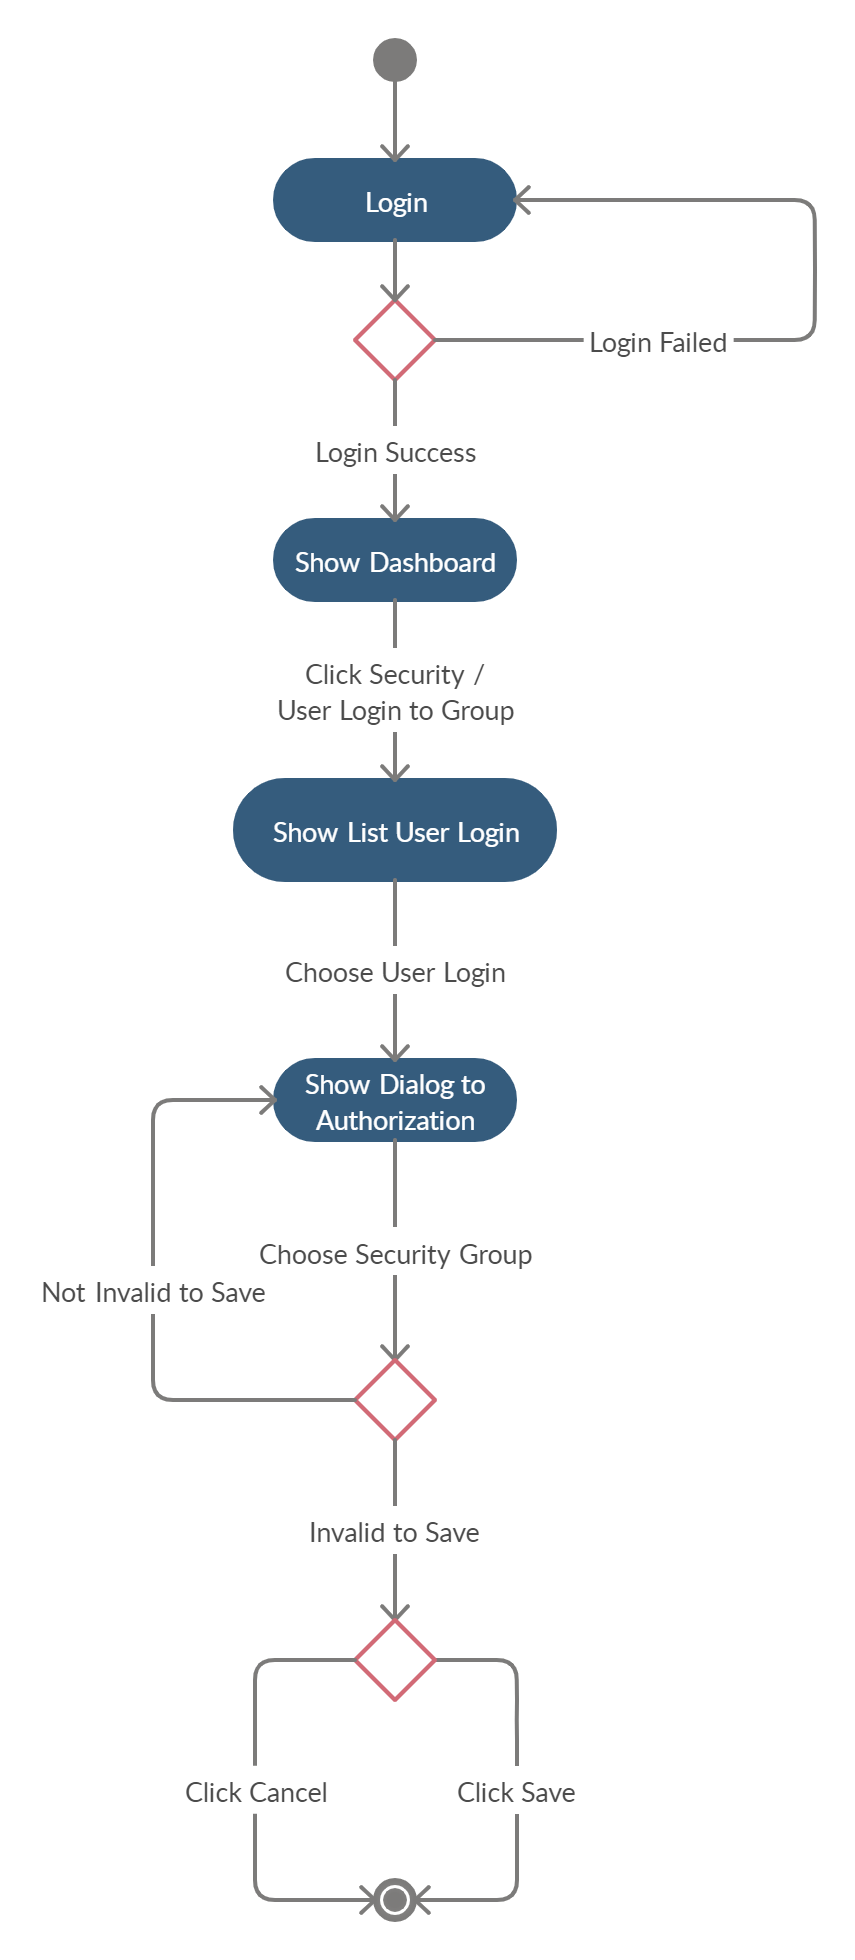
\includegraphics[width=7cm]
{images/activity-diagram/assign-permissions.png}
\caption{Biểu đồ hoạt động cho thao tác phân quyền}
\end{figure}

\subsubsection{Quản lý kho}
Biểu đồ use case cho ca sử dụng quản lý kho:
\begin{figure}[H]
\centering
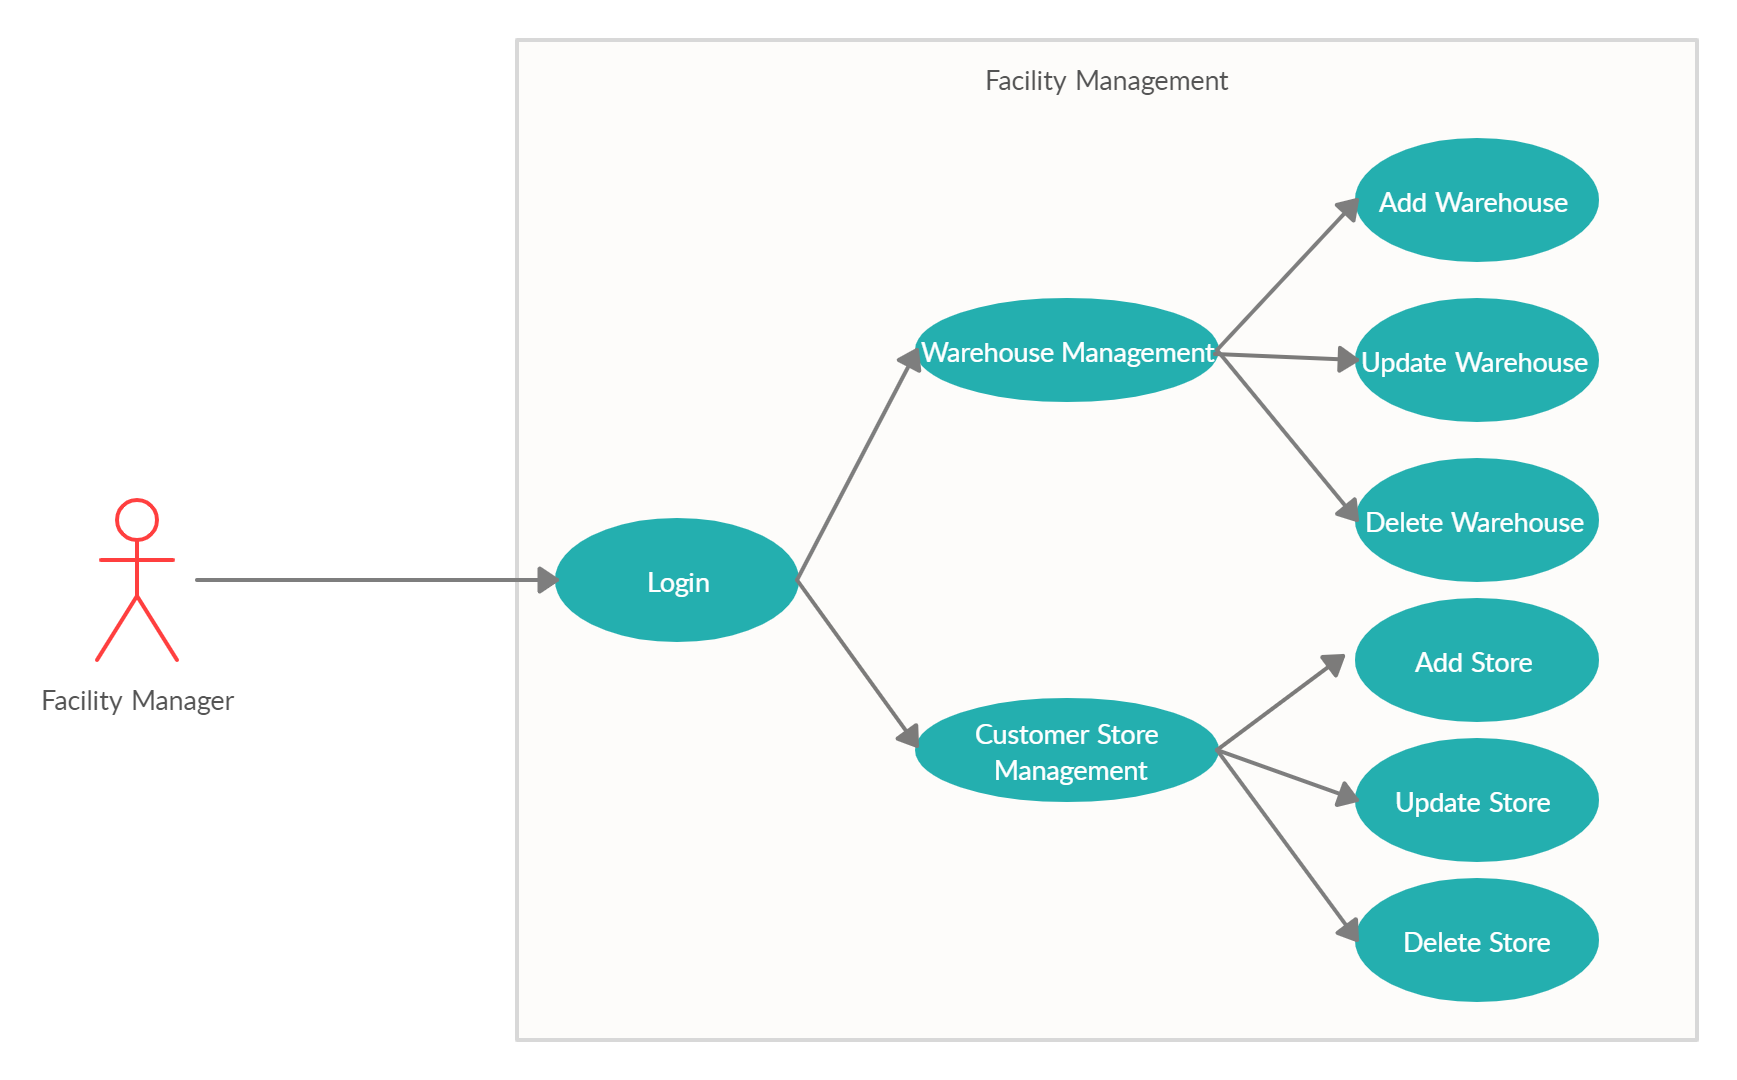
\includegraphics[width=14cm]{images/use-case/facility-management.jpg}
\caption{Use case quản lý kho}
\end{figure}

Người quản lý kho (Facility Manager) nắm được các thông tin
về kho của doanh nghiệp, tập đoàn và kho của cửa hàng bán lẻ,
có thể thêm / sửa / xóa các kho này. 

Biểu đồ hoạt động cho thao tác thêm cửa hàng bán lẻ:
